\documentclass{article}
\usepackage[utf8]{inputenc}

\usepackage{graphicx}
\usepackage[spanish, es-tabla]{babel}
\usepackage{fullpage}
\usepackage{hyperref}
\usepackage{breakurl}
\usepackage{booktabs}
\usepackage{amsmath} 

\title{Resultados finales}
\author{Ionatan Perez}
\date{October 2016}

\begin{document}

\maketitle

\section{Planteo del experimento}


El objetivo general de la tesis es identificar y estudiar que variable influyen en el reconocimiento de patrones geometricos en la representacion sonora de las mismas mediante una codificacion tipo vOICe. En trabajos preliminares observamos que dicha capacidad depende drasticamente de la orientacion de los segmentos que componen las figuras en relacion a los ejes horizontales y verticales. Por ello las mediciones que realizamos a continuacion se centraron en observar dicha capacidad en figuras cuyos segmentos estuvieran orientados lejos de los ejes. 

El experimento realizado consistió en medir el nivel de umbral de deteccion de "paralalelismo" / "no paralelismo" y de "angulo recto" / "angulo no recto" en diferentes orientaciones, antes y despues de un proceso de entrenamiento. Para eso se diseñaron ocho orientaciones (cuatro de angulos y cuatro de paralelas).

Cada orientacion esta conformado por un conjunto de estimulos diferentes donde se generan variaciones en la medida que llamaremos señal o intensidad de señal y a su vez se genera variantes para cada intensidad de señal. En el caso de paralelismo la intensidad de señal es cuanto difiere (hacia ambos lados) el angulo formado por los segmentos del caso 0, es decir dos segmentos separados pero paralelos. En el caso de los angulos se genera un angulo formado por dos lados, uno que se mantiene fijo en la direccion dada por la orientacion y otro que varia formando angulos que difieren del angulo recto en la cantidad que llamamos señal. A su vez todos estos estimulos se rotan (en conjunto, ambos segmentos) levemente (bastante menos que la diferencia entre orientacion y orientacion) de manera de que para cada intensidad de señal haya multiples estimulos posibles. A los estimulos de señal 0 (segmentos paralelos o angulos rectos), tambien los denominamos estimulos neutros o sin señal. Todas las figuras estan centradas en el lienzo.

Cada experimento o nivel consiste en escuchar el sonido correspondiente a una serie de estimulos y responder si se trata de un estimulo neutro o con señal. Mediante un algoritmo tipo escalera se elijen dinamicamente los estimulos a mostrar de manera que la dificultad de la tarea aumente o disminuya en funcion de los aciertos o errores cometidos. El objetivo de cada nivel es determinar cual es el nivel de dificulad en el cual el usuario tiene la capacidad (estadistica) de reconocer correctamente una proporcion dada de los estimulos. En otras palabras, detectar el umbral de señal en el cual el usuario pasa de distinguir la mayor parte de los estimulos a no hacerlo. 

Los niveles diseñados pueden cumplir dos funciones diferentes, ser un nivel de evaluacion de la capacidad del sujeto (niveles tipo test) o ser un nivel diseñado para entrenar al sujeto (nivel entrenamiento). La principal diferencia es que en general en estos ultimos se porporciona feedback al usuario acerca de su respuesta y su longitud.

\section{Preguntas que se buscaron estudiar}

Al ajustar los parametros de la configuracion experimental se busco poder responder las siguientes preguntas:

\begin{itemize}
    \item ¿Cuan dificil le resulta a los usuarios reconocer las figuras en diferentes orientaciones previamente a cualquier entrenamiento?
    \item ¿Como afecta el entrenamiento la capacidad de reconocimiento de los patrones?
    \item ¿El entrenamiento realizado en una orientacion y geometria especifica, se transfiere a otras orientaciones y/o orientaciones?
\end{itemize}

Para responder estas preguntas decidimos realizar en los sujetos el siguiente protocolo:

\begin{enumerate}
    \item En una primera sesion, luego de un tutorial, realizamos a todos los sujetos una evaluacion (nivel tipo test) en ocho configuraciones de orientacion-categoria diferente. Evaluamos para las orientaciones 30º, 60º 120º y 150º en las categorias paralelismo y angulos. Llamamos a estas categorias P30, P60, P120, P150 y A30, A60, A120, A150 respectivamente. El orden mencionado de los niveles se mantuvo constante en todos los sujetos.
    
    La eleccion de orientaciones fue hecha de manera de tener una gran cantidad de simetrias. Como se puede observar en las figuras \ref{fig:simetriasAngulos} y \ref{fig:simetriasParalelismo}, las orientaciones 30 y 150 y 60 y 150 son simetricas respecto a la vertical en ambas categorias. Las paralelas tambien respetan esta simetria respecto a la horizontal, mientras que los angulos respetan simetria (asumiendo el caso de estimulos con angulos cercanos al recto) respecto a la horizontal entre 30 y 60 y 120 y 150 respectivamente. A su vez la simetria entre 30 y 60 o 120 y 150 en las paralelas esta dada por la reflexion a 45º. Por otra parte todos los estimulos de paralelismo tienen simetria de rotacion, mientras que los de angulos lo hacen de a pares (30 y 60 y 120 y 150) porque se rompe la simetria completa al dejar un lado "fijo". Dado que los valores finales de umbral son grandes en comparacion con las fluctuaciones que se generan dentro de cada "lado fijo" no se puede asumir que esta simetria se restituye. 
    
    \begin{figure}
        \centering
        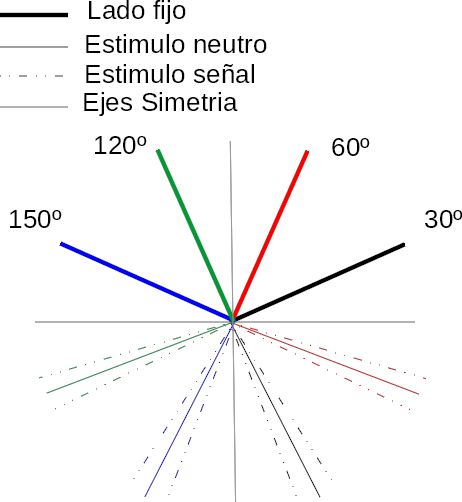
\includegraphics[width=0.3\textwidth]{Imagenes/SimetriasOrientacionAngulos.png}
        \caption{Orientaciones y simetrias para los estimulos de ángulos}
        \label{fig:simetriasAngulos}
    \end{figure}
    
        \begin{figure}
        \centering
        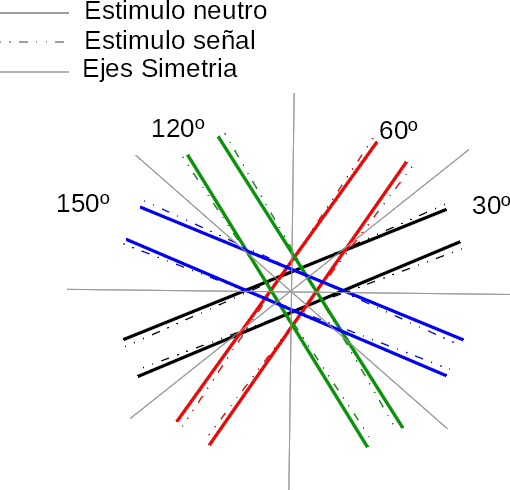
\includegraphics[width=0.3\textwidth]{Imagenes/SimetriasOrientacionParalelismo.png}
        \caption{Orientaciones y simetrias para los estimulos de paralelismo.}
        \label{fig:simetriasParalelismo}
    \end{figure}
    
    \item Entrenamos a algunos sujetos en la categoria P30 y a otros en la categoria A30. Para el entrenamiento se planeo cuatro sesiones (en dias diferentes entre si y diferentes al del test). En cada sesion se realizaron tres niveles, uno inicial con feedback, otro intermedio y mas corto sin feedback y uno final con feedback. Con este diseño se intento medir si al quitar el feedback se reducia la habilidad, si mejoraba igual o en menor medida. 
    
    \item Volvimos a realizar a todos los sujetos entrenados (y a otros tantos a modo de control) el mismo test que en la sesion inicial (sin el tutorial). 
    
\end{enumerate}

\section{Mediciones obtenidas}

    A partir del protocolo experimental diseñado se tomo datos para diez sujetos. La principal limitacion que llevo a un numero de sujetos tan bajo fue la longitud del experimento. Cada sujeto entrenado debio presentarse al laboratorio para tomas mediciones en seis oportunidades diferentes, por lo que, pese a ofrecer una retribucion economica no resulto facil conseguir sujetos que estuvieran dispuestos a participar en seis ocaciones y que tuviera compatibilidad horaria para que el experimento se dearrollara en un tiempo no extremadamente largo. 
    
    Con estas limitaciones entrenamos a dos sujetos en la categoria P30 y a dos en la categoria A30. Un quinto sujeto que no pudo completar el proceso de entrenamiento llego a hacer una sesion de entrenamiento en P30 y viendo los resultados preliminares le ofrecimos concluir el experimento en forma anticipada.
    
    Contando con estos 5 sujetos entrenados tambien medimos otros tantos sujetos a modo de control completando el conjunto de diez sujetos. 
    
    En las figuras \ref{fig:DatosTest} y \ref{fig:DatosEntrenamiento} se puede observar las medidas obtenidas para cada sujeto en cada uno de los niveles que realizo. El primer grafico muestra el desempeño para todos los sujetos, en la evaluacion previa y posterior al entrenamiento, y en el segundo grafico se muestra la evolución del sujeto a lo largo del entrenamiento para el caso de los sujetos que entrenaron.
    
    \begin{figure}
        \centering
        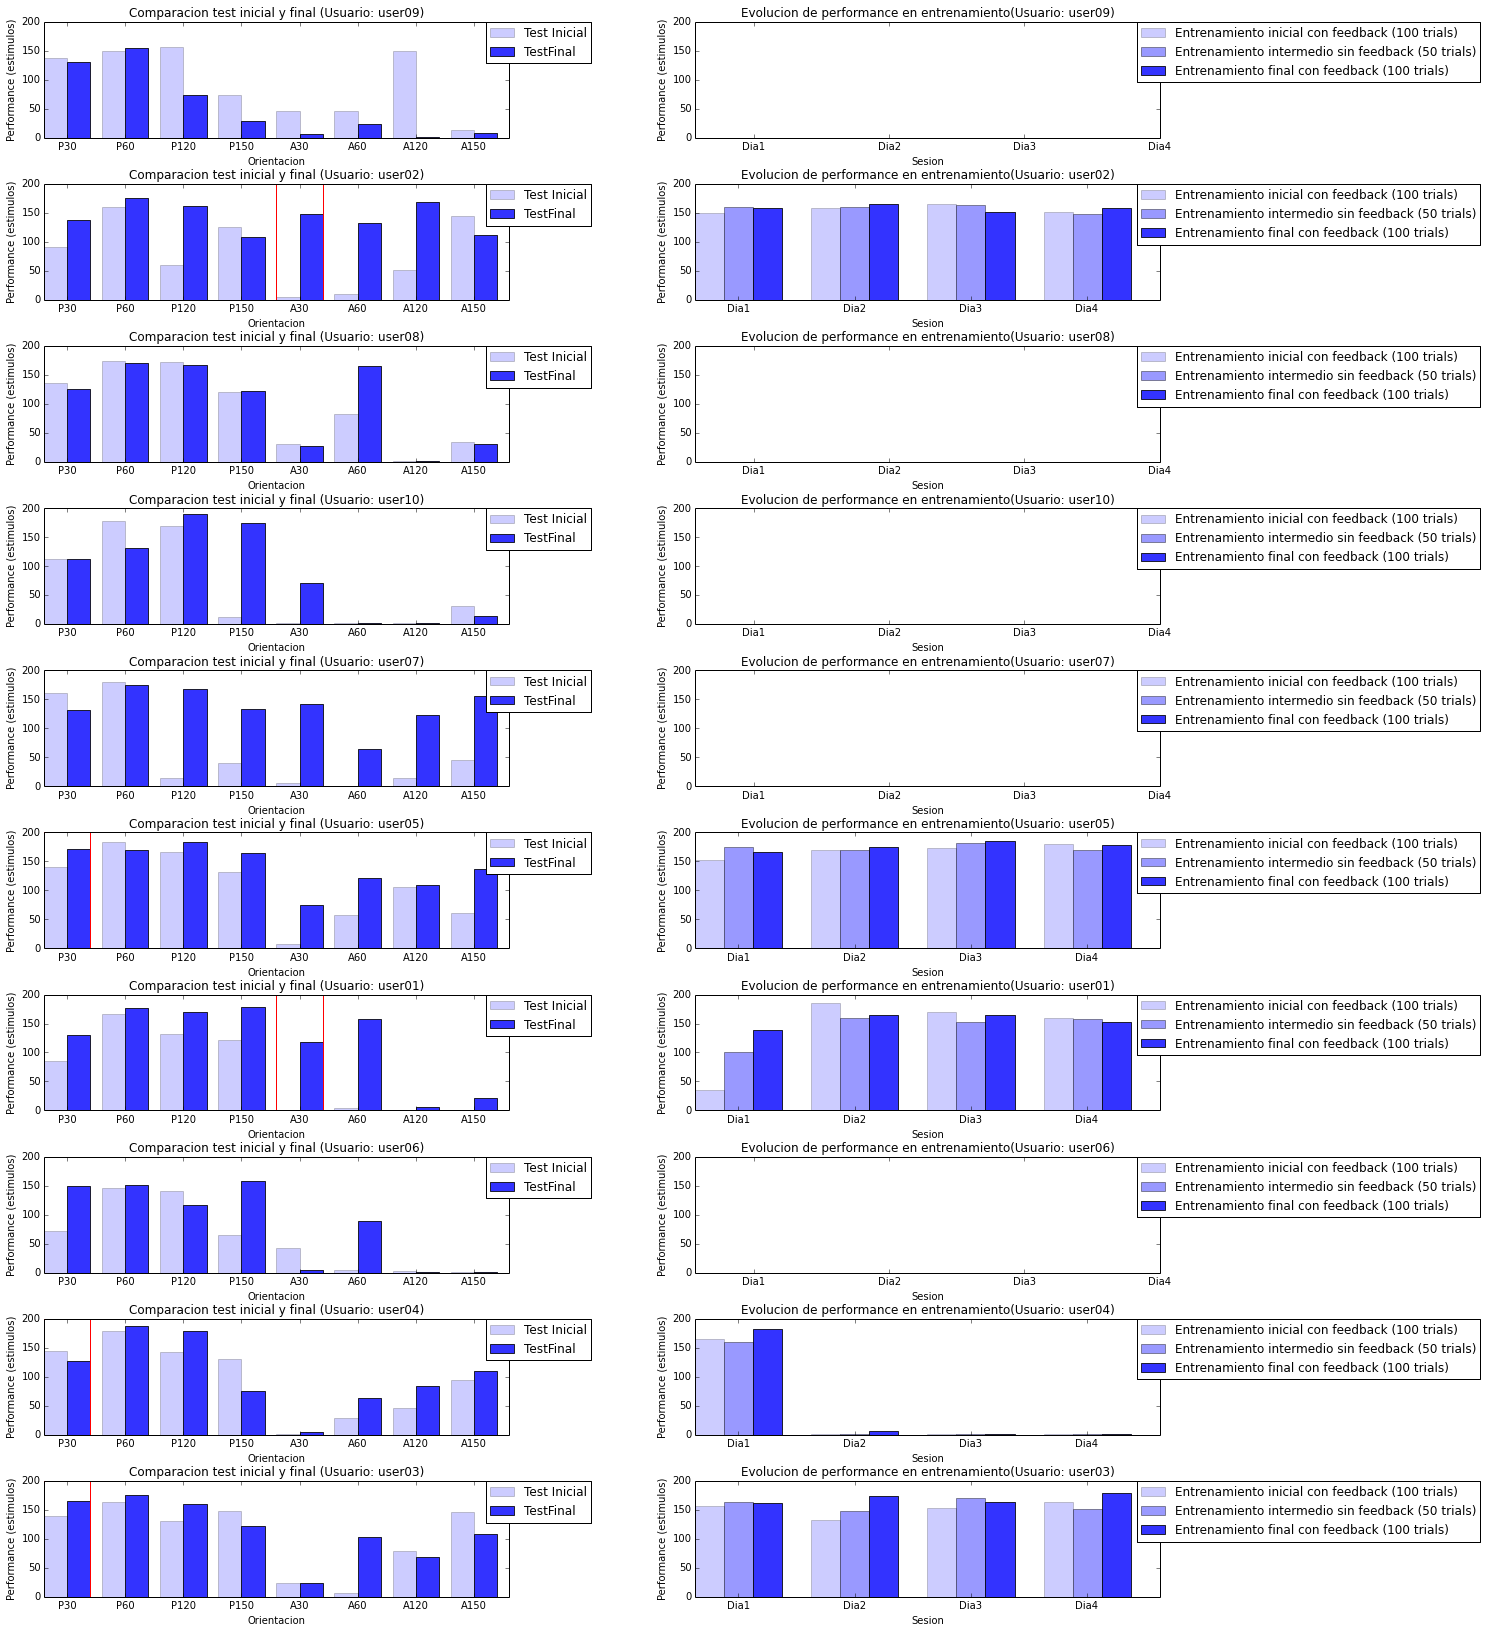
\includegraphics[width=0.9\textwidth]{Imagenes/TransferenciaResultados.png}
        \caption{Orientaciones y simetrias para los estimulos de ángulos}
        \label{fig:DatosBrutos}
    \end{figure}
    
    \begin{figure}
        \centering
        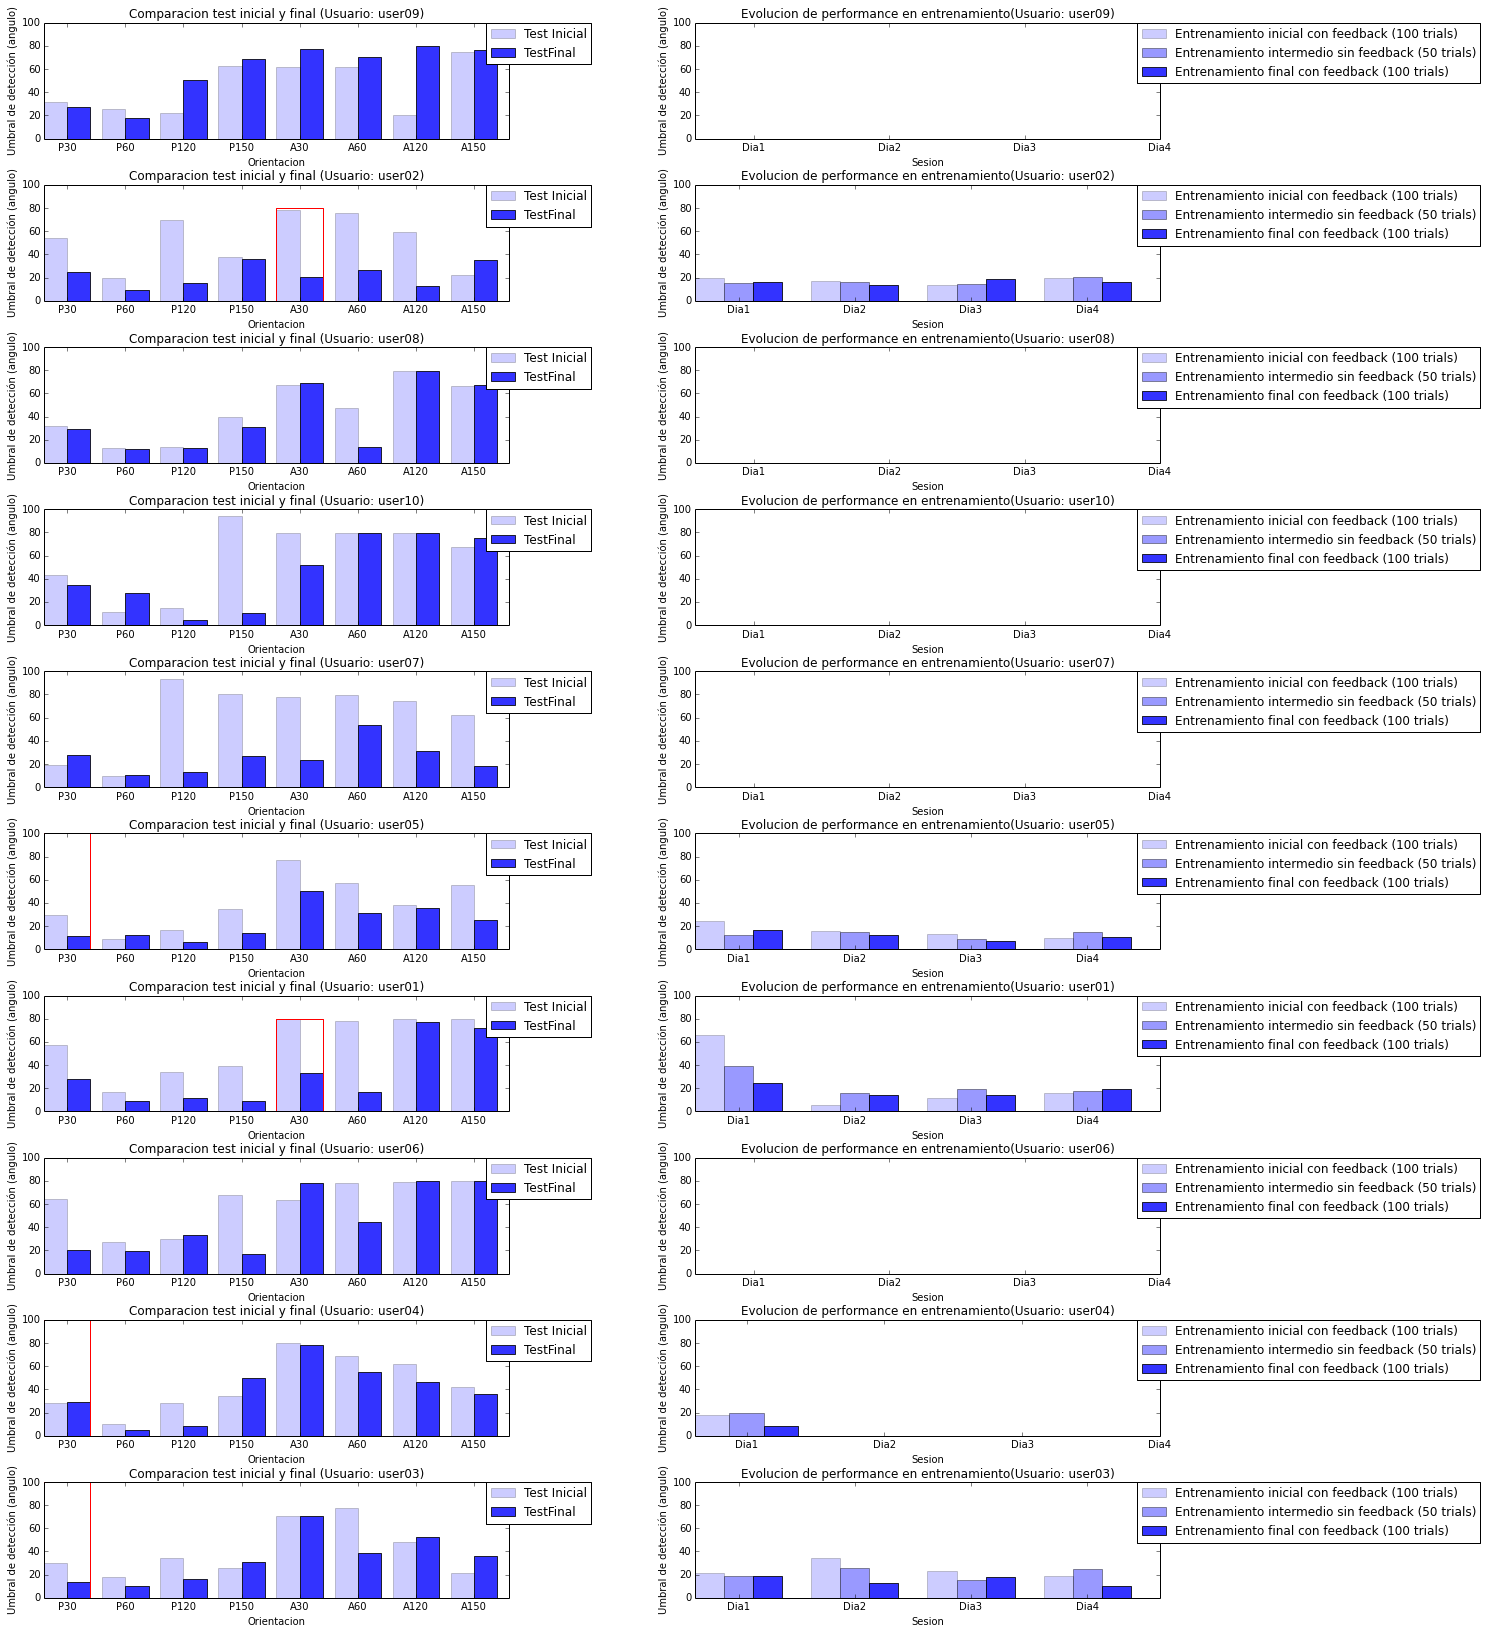
\includegraphics[width=0.9\textwidth]{Imagenes/TransferenciaResultadosEnAngulos.png}
        \caption{Orientaciones y simetrias para los estimulos de paralelismo.}
        \label{fig:DatosBrutosEnAngulos}
    \end{figure}

\section{Resultados que se derivan de las mediciones}

El primer resultado que se puede observar a simple vista es que el entrenamiento satura muy rapido. En otras palabras que los sujetos alcanzan una performance alta al concluir el primer nivel de entrenamiento (que tiene feedback) y que ese nivel se mantiene mas o menos estable a lo largo de todo el proceso posterior de entrenamiento. Esto nos lleva a hacernos la siguiente pregunta:

\textbf{¿Cuan rápido satura el entrenamiento?}

Para responder esta pregunta tomamos todas las medidas de umbral correspondientes a la categoria entrenada, separadas por sujeto. A esta secuencia de datos, los ajustamos con el siguiente modelo:

\begin{equation} \label{ec:RegresionEntrenamiento}
    Y(i,t) = \alpha_i + \beta \cdot t + \gamma_{inicial} \Theta_{inicial} + \gamma_{final} \Theta_{final}
\end{equation}

donde i representa el sujeto, t el numero de nivel (ordenados segun se realizaron), $\Theta$ un indicador de si el t corresponde al valor inicial o final de la serie (los tests), $\gamma$ el valor en que cambia el nivel medio de performance entre el test inicial o final y el entrenamiento (agrupado para todos los sujetos), $\alpha_{i}$ un factor fijo (parametro que se ajusta agrupando por categoria) que mide la performance media por sujeto, y $\beta$ la pendiente de la performance durante el entrenamiento.

Expandida para un caso de dos sesiones de entrenamiento, y tres sujetos, quedaria de la forma \ref{ec:MatrixExpandida}

\begin{equation} \label{ec:MatrixExpandida}
    \bar {Y} = \bar{\delta} \cdot \bar{\bar{X}} \text{ con } \bar{\bar{X}} =
     \begin{pmatrix}
        \beta & \alpha_1 & \alpha_2 & \alpha_3 & \gamma_{inicial} & \gamma_{final} \\
        0 & 1 & 0 & 0 & 1 & 0\\
        1 & 1 & 0 & 0 & 0 & 0\\
        2 & 1 & 0 & 0 & 0 & 0\\
        3 & 1 & 0 & 0 & 0 & 1\\
        0 & 0 & 1 & 0 & 1 & 0\\
        1 & 0 & 1 & 0 & 0 & 0\\
        2 & 0 & 1 & 0 & 0 & 0\\
        3 & 0 & 1 & 0 & 0 & 1\\
        0 & 0 & 0 & 1 & 1 & 0\\
        1 & 0 & 0 & 1 & 0 & 0\\
        2 & 0 & 0 & 1 & 0 & 0\\
        3 & 0 & 0 & 1 & 0 & 1\\
     \end{pmatrix} \text{ y $\bar{\delta}$ el conjunto de parametros buscados}
 \end{equation}

Analisando con este criterio todos los datos medidos (sin importar si entrenaron en angulos o en paralelismo o si entrenaron todas las sesiones o menos) obtenemos los resultados que se observan en la tabla \ref{tabla:entrenamientoGlobal} donde se pueden observar las siguientes conclusiones:


\begin {table}

\begin{center}

\caption{OLS Regression Results para el conjunto de todas las mediciones}
\label{tabla:entrenamientoGlobal}

\vspace{0.3in}

\begin{tabular}{lclc}

\toprule
\textbf{Dep. Variable:}    &        y         & \textbf{  R-squared:         } &     0.545   \\
\textbf{Model:}            &       OLS        & \textbf{  Adj. R-squared:    } &     0.485   \\
\textbf{Method:}           &  Least Squares   & \textbf{  F-statistic:       } &     9.068   \\
\textbf{Date:}             & Mon, 31 Oct 2016 & \textbf{  Prob (F-statistic):} &  2.61e-07   \\
\textbf{Time:}             &     15:34:05     & \textbf{  Log-Likelihood:    } &   -279.94   \\
\textbf{No. Observations:} &          61      & \textbf{  AIC:               } &     575.9   \\
\textbf{Df Residuals:}     &          53      & \textbf{  BIC:               } &     592.8   \\
\textbf{Df Model:}         &           7      & \textbf{                     } &             \\
\bottomrule
\end{tabular}

\begin{tabular}{lccccc}
            & \textbf{coef} & \textbf{std err} & \textbf{t} & \textbf{P$>|$t$|$} & \textbf{[95.0\% Conf. Int.]}  \\
\midrule
\textbf{$\beta$} &       2.6804  &        1.037     &     2.584  &         0.013        &         0.599     4.761       \\
\textbf{$\alpha_1$} &     147.9547  &        9.683     &    15.281  &         0.000        &       128.534   167.375       \\
\textbf{$\alpha_2$} &     135.2405  &        9.683     &    13.967  &         0.000        &       115.820   154.661       \\
\textbf{$\alpha_3$} &     159.8119  &        9.683     &    16.505  &         0.000        &       140.391   179.233       \\
\textbf{$\alpha_4$} &     121.9547  &        9.683     &    12.595  &         0.000        &       102.534   141.375       \\
\textbf{$\alpha_5$} &     168.6959  &       12.158     &    13.876  &         0.000        &       144.311   193.081       \\
\textbf{$\gamma_i$} &     -60.7316  &       13.418     &    -4.526  &         0.000        &       -87.644   -33.819       \\
\textbf{$\gamma_f$} &     -30.5521  &       13.418     &    -2.277  &         0.027        &       -57.465    -3.640       \\
\bottomrule
\end{tabular}

\begin{tabular}{lclc}
\textbf{Omnibus:}       & 19.666 & \textbf{  Durbin-Watson:     } &    1.279  \\
\textbf{Prob(Omnibus):} &  0.000 & \textbf{  Jarque-Bera (JB):  } &   37.440  \\
\textbf{Skew:}          & -1.013 & \textbf{  Prob(JB):          } & 7.41e-09  \\
\textbf{Kurtosis:}      &  6.259 & \textbf{  Cond. No.          } &     41.9  \\
\bottomrule
\end{tabular}
\end{center}

\end{table}

De este ajuste se puede observa las siguientes conclusiones:

\begin{itemize}
    \item Todos los parametros dieron significativos ($p<0.05$) esto significa que hay un salto entre el nivel inicial y el entrenamiento, entre el del test final y el entrenamiento y ademas a lo largo del entrenamiento hubo una mejora, sin embargo los unicos dos parametros cuyo p valor dio numericamente distinto de cero fueron el $\beta$ y el $\gamma_f$. Esto significa que son los efectos menos marcados.
    \item El parametro $\beta$ dio significativo pero muy chico. Es veinte veces menor que el $\gamma_i$, lo cual nos dice que la mejora promedio entre nivel y nivel (posterior al inicial) es veinte veces menor a la mejora tras el primer entrenamiento con feedback, esto indica una mejora cuantitativa mas que cualitativa al realizar entrenamiento, que probablemente tenga que ver con un cambio conceptual en el entendimiento de la tarea a realizar. Tambien indica que se debe tener cuidado en realizar controles acerca del entrenamiento durante el primer test aunque los test se realicen en diferentes categorias.
    \item El parametro $\gamma_f$ dio aproximadamente la mitad que el $\gamma_i$. Si descontamos el efecto de entrenamiento, significa que la performance empeora al realizar una evaluacion sin feedback pero no tanto como para regresar al nievel inicial. Igual para comprobar esta ultima hipotesis tiene sentido hacer un test aparte. Se debe considerar el hecho de que el test final se realiza en un contexto diferente al entrenamiento y que no tiene feedback. 
\end{itemize}

Sin embargo, mirando los datos en bruto se observa que hay un sujeto que presenta una clara evolucion en su progreso durante el primer dia de entrenamiento, y dado el bajo numero de sujetos puede estar afectando toda la medida. Si repetimos el mismo ajuste pero tomando solo los datos de entrenamiento del segundo dia en adelante (lo cual tambien descarta al sujeto que entreno un solo dia), obtenemos los resultados que se observan en la tabla \ref{tabla:entrenamietoParteFinal} donde se puede ver que el valor de $\beta$ no es significativamente distinto de 0 (con mucho margen), por ende podemos decir que claramente no hay entrenamiento del segundo dia en adelante. De hecho, repitiendo el analisis inicial pero descartando al sujeto que muestra una mejora en la primer sesion, el p valor de $\beta$ da 0.119, es decir que sin considerar ese sujeto tampoco se ve un efecto de aprendizaje a lo largo del entrenamiento (salvo el contraste ya mencionado entre el umbral antes y despues del primer nivel con feedback). 

\begin {table}

\begin{center}

\caption{OLS Regression Results para el los dias 2, 3 y 4 de entrenamiento}
\label{tabla:entrenamietoParteFinal}
\vspace{0.3in}

%\begin{tabular}{lclc}
%\toprule
%\textbf{Dep. Variable:}    &        y         & \textbf{  R-squared:         } &     0.356   \\
%\textbf{Model:}            &       OLS        & \textbf{  Adj. R-squared:    } &     0.273   \\
%\textbf{Method:}           &  Least Squares   & \textbf{  F-statistic:       } &     4.292   \\
%\textbf{Date:}             & Mon, 31 Oct 2016 & \textbf{  Prob (F-statistic):} &  0.00704    \\
%\textbf{Time:}             &     17:12:46     & \textbf{  Log-Likelihood:    } &   -132.13   \\
%\textbf{No. Observations:} &          36      & \textbf{  AIC:               } &     274.3   \\
%\textbf{Df Residuals:}     &          31      & \textbf{  BIC:               } &     282.2   \\
%\textbf{Df Model:}         &           4      & \textbf{                     } &             \\
%\bottomrule
%\end{tabular}

\begin{tabular}{lccccc}
            & \textbf{coef} & \textbf{std err} & \textbf{t} & \textbf{P$>|$t$|$} & \textbf{[95.0\% Conf. Int.]}  \\
\midrule
\textbf{$\beta$} &       0.0625  &        0.661     &     0.095  &         0.925        &        -1.285     1.410       \\
\textbf{$\alpha_1$} &     159.3056  &        4.317     &    36.902  &         0.000        &       150.501   168.110       \\
\textbf{$\alpha_2$} &     157.8611  &        4.317     &    36.567  &         0.000        &       149.057   166.666       \\
\textbf{$\alpha_3$} &     175.7500  &        4.317     &    40.711  &         0.000        &       166.945   184.555       \\
\textbf{$\alpha_4$} &     162.5278  &        4.317     &    37.648  &         0.000        &       153.723   171.332       \\
\bottomrule
\end{tabular}

%\begin{tabular}{lclc}
%\textbf{Omnibus:}       &  2.518 & \textbf{  Durbin-Watson:     } &    1.645  \\
%\textbf{Prob(Omnibus):} &  0.284 & \textbf{  Jarque-Bera (JB):  } &    1.526  \\
%\textbf{Skew:}          &  0.003 & \textbf{  Prob(JB):          } &    0.466  \\
%\textbf{Kurtosis:}      &  4.009 & \textbf{  Cond. No.          } &     17.7  \\
%\bottomrule
%\end{tabular}

\end{center}

\end{table}

Sin embargo todo el analisis realizado habla de una evolucion intrasujeto, pero no discrimina entre las mediciones realizadas en paralelismo y las mediciones realizadas en angulos.

\textbf{¿Son comparables las medidas en angulos y las medidas en paralelismo?}

A priori no tendrian porque serlo. Son tests que miden habilidades diferentes, que si bien comparten el metodo de medicion utilizan escalas diferentes por medir dos caracteristicas intrisicamente diferentes. Ademas no esta claro a que se define como dificultad mas alla de observar una mejora o no en la variable medida al realizar el entrenamiento. Por lo tanto no tiene sentido comparar ambas medidas. Como prueba de ello, el la figura \ref{fig:equivalencia} se puede observar la comparacion del valor medio en todas las medidas tomadas con los sujetos entrenados (asumimos en base a lo discutido anteriormente que el entrenamiento satura en el primer nivel) en un categoria con los entrenados en la otra. Hacemos la comparacion utilizando un mannwhitneyu u test en la escala arbitraria en que se mide la performance y en la escala que corresponde al angulo absoluto. Se puede observar que no hay diferencias significativas en una escala y si en la otra (los p value fueron 0.012 y 0.218). El hecho de que el cambio de escalas afecte la significancia de comparar ambos conjuntos de medidas esta relacionado a que cada categoria tiene su propia factor de transformacion. 

De esta figura se podria concluir que la dificultad para detectar las categorias mencionadas es similar al menos medida en terminos absolutos, pero lo cierto es que la propia escala absoluta es arbitraria, en tanto el angulo formado por los dos segmentos se puede medir como el angulo entre ellos o el angulo respecto a la mediatriz, solo por mencionar un ejemplo.

\begin{figure}
        \centering
        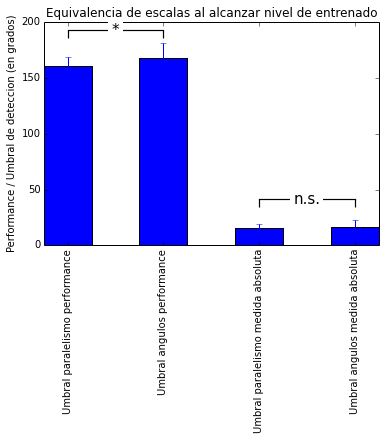
\includegraphics[width=0.5\textwidth]{Imagenes/EquivalenciaDeEscalas.png}
        \caption{Comparacion entre los niveles de umbral alcanzados por los sujetos entrenados en paralelismo y en angulos medido en terminos de la performance y del angulo formado en la figura.}
        \label{fig:equivalencia}
\end{figure}

\textbf{¿Afecta el feedback o la repeticion de los niveles en una misma sesion a la performance?}

El diseño del experimento se hizo para que cada sesion tuviera un nivel largo con feedback, uno corto sin feedback y uno final igual al inicial. Ademas, cada uno de los segundos y terceros niveles de cada sesion comienza en el nivel de dificultad que concluyo el anterior de manera de evitar efectos debido a diferentes procesos de convergencia del algoritmo dinamico que regula la dificultad. 

El objetivo de este diseño era observar si se producia una reduccion de la performance al quitar el feedback y ademas observar si habia una mejora intra sesion producto del entrenamiento. Esta mejora podria encuadrarse en el marco de una mejora global inter sesion, pero como mostramos con anterioridad, este efecto no se oberva si descartamos la unica sesion donde un sujeto mostro una progresion marcada. Por esta razon al evaluar la mejora intra sesion se estaria evaluando si hay un efecto de "olvido" entre sesion y sesion que se revierta durante la misma. 

Para analizar esta posible mejora, se considero cuatro criterios diferentes. Agrupar todos los valores de entrenamiento inicial, medio y final, sin importar la sesion de la que provienen. Agregar un factor fijo por usuario, agregar un factor fijo por dia, o agregar ambos factores. Este ultimo caso lo que hace es restar el valor medio de cada sesion al conjunto de datos. La ventaja de agregar factores fijos es que permite identificar posibles parametros que distingan efectos, pero aumenta el rango de error del conjunto de los parametros calculados. En cualquiera de los casos, dio que la pendiente de aprendizaje no es significativa. 




\begin{table}

\begin{center}

\caption{OLS Regression: pendiente de aprendizaje intrasesion ajustada con diferentes criterios}
\label{tabla:betasIntrasesion}
\vspace{0.3in}

\begin{tabular}{lccccc}
            Criterio & valor & \textbf{std err} & \textbf{t} & \textbf{P$>|$t$|$} & \textbf{[95.0\% Conf. Int.]}  \\
\midrule
$\beta$ Sin efecto fijo &       3.0625  &       1.965     &     1.559  &         0.126       &        -0.893     7.018       \\
$\beta$ Efecto fijo por sujeto &  3.0625    &  1.704    &  1.797    &  0.079    &    -0.376     6.501\\
$\beta$ Efecto fijo por dia &     3.0625    &  2.013    &  1.522    &  0.135    &    -0.997     7.122\\
$\beta$ Efecto fijo por sesion &    3.0625  &    1.723  &    1.777  &    0.083  &      -0.422     6.547 \\
$\beta$ Efecto fijo para segundo nivel & 3.0625 &     1.725 &     1.776 &     0.084     &   -0.429     6.554 \\
Parametro del efecto fijo para segundo nivel & -2.8750    &  3.414 &     -0.842 &     0.404   &     -9.752     4.002 \\
\bottomrule
\end{tabular}

\end{center}

\end{table}

\end{document}
